\subsection{Single-date comparison across backbones and cohorts}
Table~\ref{tab:backbone_cohort} uses the same AP contrast in all four cells. The gain over ordinary self-training was 12.17--14.15 AP points on ImpactMesh and 0.17--1.19 points on GEOID-Flood. The original GEOID-Flood U-Net primary contrast remains the comparison with same-rule post-processing. It yielded a gain of 3.50 AP points (eight of nine activations, one-sided exact sign test $p=0.0195$). Ordinary self-training was the secondary comparator.

\begin{table}[pos=t]
\centering
\caption{Joint physics-guided versus ordinary self-training in the single-date evaluations. AP values are percentages, and gains are percentage points calculated before rounding. Metrics average three source checkpoints within each activation and then weight activations equally. Both ImpactMesh rows and the ResNet-50 GEOID-Flood row use the post-hoc crossover runs.}
\label{tab:backbone_cohort}
\begin{tabular}{@{}llrrrr@{}}
\toprule
Cohort & Backbone & Ordinary AP & Joint AP & Gain & Wins \\
\midrule
ImpactMesh & U-Net & 47.91 & 60.09 & +12.17 & 12/13 \\
ImpactMesh & SSL4EO ResNet-50 & 45.81 & 59.95 & +14.15 & 12/13 \\
GEOID-Flood & U-Net & 67.75 & 67.91 & +0.17 & 8/9 \\
GEOID-Flood & SSL4EO ResNet-50 & 66.39 & 67.58 & +1.19 & 8/9 \\
\bottomrule
\end{tabular}
\end{table}

\subsection{ImpactMesh-Flood: incremental value of physical cues}
\label{sec:external}

The paired AP gain on ImpactMesh had a median of 4.24 points, with improvements on 12 of 13 activations (one-sided exact sign test, $p=0.00171$). Mean AP rose from 45.10\% to 60.03\%, with a mean gain of 14.93 points (post-hoc 95\% bootstrap interval 6.67--24.30 points). Four activations contributed 76\% of the net gain. The exploratory two-sided signed-rank result is reported with the archived-score diagnostics. On EMSR795, misses fell from 99.47\% to 18.06\%. On EMSR799, misses fell from 100.00\% to 40.97\%, but FPR rose by 25.18 points and AP remained near 2\% (Fig.~\ref{fig:impactmesh_paired}).

At the 0.430 source threshold, mean IoU rose from 25.96\% to 42.01\% and the mean miss rate fell from 60.08\% to 28.88\% (Table~\ref{tab:impactmesh}). Dry-pixel FPR increased on all 13 activations. On the nine activations with defined FDP for every seed in both arms, mean FDP was 40.32\% for ordinary self-training and 39.38\% for physics-guided self-training. For physics-guided self-training, FDP was defined on all 13 activations and averaged 47.32\%.

At matched FPR, physics improved recall over ordinary self-training on 12 of 13 activations at 2\% FPR and 11 of 13 at 5\% FPR. The event-level scatterplots put the ImpactMesh AP gains alongside the smaller GEOID-Flood changes (Fig.~\ref{fig:external_review_events}), and the macro precision--recall curves show how precision changes across matched recall levels in each cohort (Fig.~\ref{fig:external_review_pr}).

\paragraph{Post-hoc inference controls.} On the same ImpactMesh activations, ordinary self-training reached 45.10\% AP, close to the source model at 44.64\% and below AdaBN at 46.04\%. Physics-guided self-training exceeded the source model by 15.39 AP points (13 of 13 activations), AdaBN by 13.99 points (12 of 13), and same-rule post-processing by 10.24 points (13 of 13). The median gains were 10.73, 9.71 and 8.36 points, respectively. At the fixed threshold, the physics arm had higher IoU and fewer misses than all three controls, with higher mean FPR. Table~\ref{tab:impactmesh_inference} reports the complete comparison.

The controls also show that ordinary self-training amplified under-detection in individual events. On EMSR795, misses were 95.74\% for the source model and 86.84\% after AdaBN, rising to 99.47\% after ordinary self-training. Physics reduced the miss rate to 18.06\%, compared with 73.85\% for same-rule post-processing. On EMSR799, ordinary self-training also missed more floodwater than either the source or AdaBN, and the physics arm's AP remained low. Median elapsed CPU time per activation--seed pair was 3.3\,s for source inference and 30.9\,s for AdaBN with inference and score collection. These timings exclude input loading and metric computation.

At 2\% and 5\% matched FPR, physics achieved 56.68\% and 72.42\% mean recall. Its nearest control, same-rule post-processing, reached 43.88\% and 57.02\%. Physics improved recall over post-processing and the source model on 12 of 13 activations at each budget, and over AdaBN on 11 of 13 at 2\% FPR and 12 of 13 at 5\% FPR. These retrospective comparisons use reference dry pixels to match false-alarm rates.

\begin{table}[pos=t]
\centering
\caption{ImpactMesh-Flood paired comparison on 13 activations. Rows report means over activations after averaging three model seeds within each activation. Percentage-point differences are physics-guided minus ordinary self-training.}
\label{tab:impactmesh}
\begin{tabular}{@{}lrrr@{}}
\toprule
Metric (\%) & Ordinary & Physics-guided & Difference \\
\midrule
Floodwater AP & 45.10 & 60.03 & $+14.93$ \\
\addlinespace
IoU at 0.430 & 25.96 & 42.01 & $+16.05$ \\
Miss rate at 0.430 & 60.08 & 28.88 & $-31.20$ \\
Dry-pixel FPR at 0.430 & 1.96 & 5.89 & $+3.93$ \\
\addlinespace
Recall at matched 2\% FPR & 39.31 & 56.68 & $+17.37$ \\
Recall at matched 5\% FPR & 52.90 & 72.42 & $+19.52$ \\
\bottomrule
\end{tabular}
\end{table}

\begin{table}[pos=t]
\centering
\caption{ImpactMesh-Flood inference controls added post hoc, alongside the original self-training arms. Means weight the 13 activations equally after averaging three seeds per activation. IoU, miss and dry-pixel FPR use the common source threshold 0.430. The last two columns report recall in percent, interpolated at target-label FPR budgets of 2\% and 5\% for each activation and seed.}
\label{tab:impactmesh_inference}
\begin{tabular}{@{}p{.32\linewidth}rrrrrr@{}}
\toprule
 & & \multicolumn{3}{c}{Source threshold} & \multicolumn{2}{c}{Matched FPR} \\
\cmidrule(lr){3-5}\cmidrule(lr){6-7}
Method & AP (\%) & IoU (\%) & Miss (\%) & FPR (\%) & Rec. at 2\% & Rec. at 5\% \\
\midrule
Source only & 44.64 & 25.92 & 57.01 & 4.36 & 36.79 & 52.54 \\
AdaBN & 46.04 & 27.35 & 54.31 & 3.11 & 39.18 & 54.30 \\
Same-rule post-processing after AdaBN & 49.79 & 30.51 & 48.84 & 3.50 & 43.88 & 57.02 \\
Ordinary self-training & 45.10 & 25.96 & 60.08 & 1.96 & 39.31 & 52.90 \\
Physics-guided self-training & 60.03 & 42.01 & 28.88 & 5.89 & 56.68 & 72.42 \\
\bottomrule

\end{tabular}
\end{table}

\begin{figure}[pos=H]
\centering
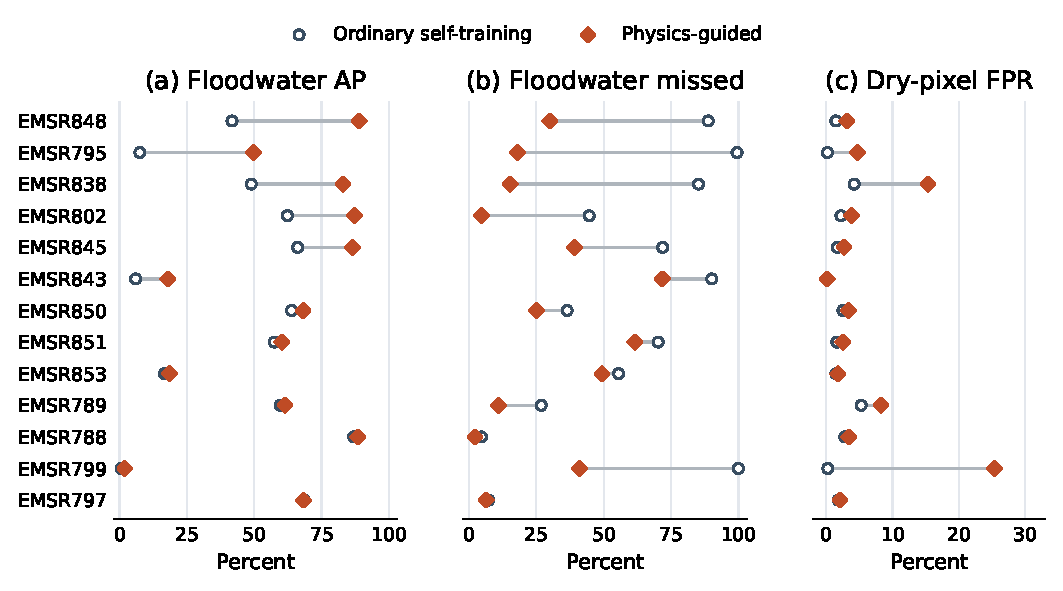
\includegraphics[width=\textwidth]{figures/fig_impactmesh_paired.pdf}
\caption{Matched ImpactMesh results for all 13 floods, ordered by AP gain. Each point averages three seeds. Miss and false-alarm rates use the common source-selected threshold of 0.430.}
\label{fig:impactmesh_paired}
\end{figure}

\begin{figure}[pos=H]
\centering
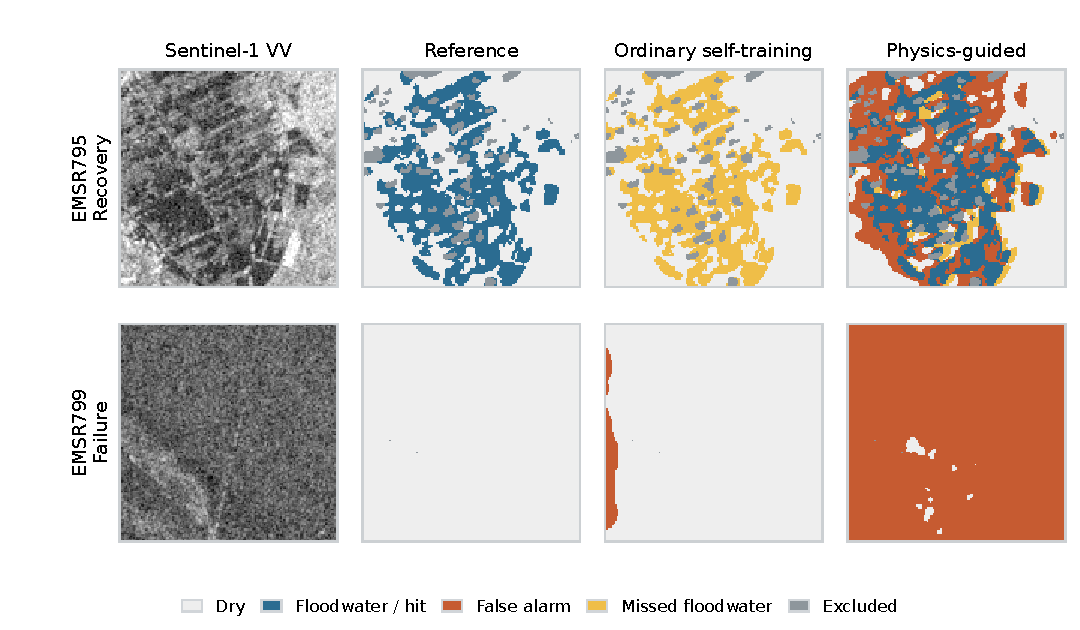
\includegraphics[width=\textwidth]{figures/fig_impactmesh_examples.pdf}
\caption{Illustrative ImpactMesh cases from the frozen scores, model seed 0 and threshold 0.430. For EMSR795 we show the chip with the largest net increase in correctly detected flood pixels. For EMSR799 we show the chip with the largest net increase in false flood pixels. These outcome-selected chips illustrate the respective effects. Grey marks excluded pixels, including permanent water. Both rows use the same VV display range, \mbox{$-26$ to $-4$\,dB}.}
\label{fig:impact_examples}
\end{figure}

Fig.~\ref{fig:impact_examples} shows how similar changes in mapped area can have very different consequences. On the selected EMSR795 chip, ordinary self-training detected none of the 20,673 labelled flood pixels. Physics detected 17,770 and also flagged 18,162 dry pixels. The selected EMSR799 chip contains no scored flood pixels. Physics marked 64,854 dry pixels as flooded, compared with 2,072 for ordinary self-training. The per-activation comparison in Fig.~\ref{fig:impactmesh_paired} shows their wider context.

Table~\ref{tab:model_free_radar} compares the standalone radar masks with physics-guided self-training on the frozen floodwater-only pixels. The adaptive VV+VH mask had low FPR and missed 73.07\% of floodwater. The VV Otsu mask missed 17.86\% at the cost of 28.19\% FPR. Physics-guided self-training achieved higher IoU than either standalone mask at the evaluated operating points.

\begin{table}[pos=t]
\centering
\caption{Post-hoc model-free radar controls and the archived physics-guided self-training result. Each mask uses its own input-derived threshold. The network uses its source-calibrated threshold. All metrics weight activations equally.}
\label{tab:model_free_radar}
\begin{tabular}{@{}llrrr@{}}
\toprule
Cohort & Method & IoU (\%) & Miss (\%) & FPR (\%) \\
\midrule
ImpactMesh & Adaptive VV+VH mask & 21.87 & 73.07 & 2.28 \\
 & VV Otsu mask & 25.42 & 17.86 & 28.19 \\
 & Physics-guided self-training & 42.01 & 28.88 & 5.89 \\
\midrule
GEOID-Flood & Adaptive VV+VH mask & 35.80 & 60.11 & 0.42 \\
 & VV Otsu mask & 24.50 & 25.89 & 20.64 \\
 & Physics-guided self-training & 43.20 & 26.19 & 4.41 \\
\bottomrule
\end{tabular}
\end{table}

\subsection{ImpactMesh single-date crossover: darkness and terrain}
\label{sec:darkness_crossover}
Adaptive darkness without terrain gates improved AP over ordinary self-training by 13.93 points on ResNet-50 (95\% paired bootstrap interval 5.54 to 23.34) and 12.30 points on U-Net (3.84 to 22.14). Adding the terrain gates changed AP by +0.22 points on ResNet-50 ($-0.17$ to 0.80) and $-0.12$ points on U-Net ($-0.30$ to 0.01). The terrain gates lowered the mean fixed-threshold FPR and slightly increased the mean miss rate on both backbones relative to darkness alone (Table~\ref{tab:darkness_crossover}).

\begin{table}[pos=t]
\centering
\caption{Post-hoc single-date crossover on 13 ImpactMesh activations. Results are percentages. We average the three seeds within each activation and weight the activations equally. Decision metrics use the source threshold of 0.430 for ResNet-50 and 0.208 for U-Net.}
\label{tab:darkness_crossover}
\begin{tabular}{@{}llrrrr@{}}
\toprule
Backbone & Self-training arm & AP & IoU & Miss & FPR \\
\midrule
ResNet-50 & Ordinary & 45.81 & 26.90 & 59.13 & 1.97 \\
          & Darkness only & 59.73 & 41.80 & 27.48 & 6.28 \\
          & Radar and terrain & 59.95 & 42.17 & 28.53 & 5.95 \\
\addlinespace
U-Net & Ordinary & 47.91 & 29.27 & 51.14 & 3.09 \\
      & Darkness only & 60.21 & 41.42 & 22.23 & 7.47 \\
      & Radar and terrain & 60.09 & 41.47 & 22.91 & 7.21 \\
\bottomrule
\end{tabular}
\end{table}

\subsection{ImpactMesh robustness to teacher cutoff and acquisition timing}
In the post-hoc ResNet-50 control, changing the teacher's positive cutoff from $p>0.90$ to $p>0.70$ improved AP by 2.67 points over the earlier ordinary Kaggle T4 run and reduced misses by 17.98 points at the source threshold. Dry-pixel FPR rose by 3.40 points. On the same GPU and software stack, joint physics exceeded the relaxed control in AP on all 13 activations, with a mean gain of 11.47 points (95\% paired activation bootstrap interval 4.94 to 19.13). At matched 2\% and 5\% FPR, joint physics gained 11.91 and 13.33 recall points, respectively (Table~\ref{tab:relaxed_control}). The comparison tests one lower teacher cutoff.

\begin{table}[pos=t]
\centering
\caption{Post-hoc ImpactMesh ResNet-50 teacher-cutoff control on the same Kaggle T4 stack. Values are percentages. Miss and FPR use the common source threshold 0.430. Matched recall is interpolated retrospectively from each activation--seed ROC curve.}
\label{tab:relaxed_control}
\begin{tabular}{@{}lrrrrr@{}}
\toprule
Method & AP & Miss & FPR & Recall at 2\% FPR & Recall at 5\% FPR \\
\midrule
Ordinary ($p>0.90$) & 45.81 & 59.13 & 1.97 & 40.91 & 54.26 \\
Relaxed ordinary ($p>0.70$) & 48.48 & 41.16 & 5.38 & 44.48 & 58.64 \\
Joint physics & 59.95 & 28.53 & 5.95 & 56.39 & 71.97 \\
\bottomrule
\end{tabular}
\end{table}

In a separate post-hoc sensitivity analysis of the original frozen ImpactMesh scores, restricting scoring to chips acquired within three days of activation and excluding EMSR848 gave a mean gain of 13.68 AP points, a median gain of 7.63 points and improvements on 10 of 11 scorable activations (Appendix~\ref{sec:acquisition_timing}). The filter used acquisition timing and did not re-run adaptation.

\subsection{ImpactMesh paired-input comparison with TG-TTA}
\label{sec:matched_tg_tta}
Across the same 13 activations, TG-TTA reached 56.92\% AP, and the VV-only and VV+VH physics arms reached 57.27\% and 58.09\% (Table~\ref{tab:tg_fixed}). The paired AP gains over TG-TTA were 0.35 points (95\% interval $-3.57$ to 4.15) and 1.17 points ($-1.37$ to 3.60). At 0.5, both physics arms lowered the miss rate and increased the dry-pixel FPR on every activation. The VV-only arm reduced the mean miss rate by 34.77 points and increased FPR by 11.04 points.

\begin{table}[pos=t]
\centering
\caption{Paired-input STANet comparison with TG-TTA on ImpactMesh. Results are percentages averaged across 13 activations after averaging the three seeds. Miss and FPR use the same source-calibrated probability threshold of 0.5.}
\label{tab:tg_fixed}
\begin{tabular}{@{}lrrr@{}}
\toprule
Method & Floodwater AP & Miss & Dry-pixel FPR \\
\midrule
Source inference & 52.46 & 62.74 & 1.86 \\
Ordinary self-training & 55.24 & 66.98 & 2.36 \\
TG-TTA port & 56.92 & 66.68 & 1.65 \\
Physics self-training (VV) & 57.27 & 31.91 & 12.69 \\
Physics self-training (VV+VH) & 58.09 & 38.00 & 9.33 \\
\bottomrule
\end{tabular}
\end{table}

Matching false alarms to TG-TTA within each activation and seed yielded a cohort mean FPR of 1.65\%. At that budget, neither physics variant reduced mean misses. The VV+VH rule missed less floodwater on eight activations, with larger losses on some of the remaining floods (Table~\ref{tab:tg_matched}). The deterministic sensitivity that excludes partially matched score ties reached the same conclusion.

\begin{table}[pos=t]
\centering
\caption{Post-hoc comparison at equal false alarms. Each physics arm matches TG-TTA's false-positive count within activation and seed. The cohort mean FPR is 1.65\%. The paired bootstrap interval is in percentage points.}
\label{tab:tg_matched}
\begin{tabular}{@{}lrrr@{}}
\toprule
Method & Miss (\%) & $\Delta$ miss (95\% interval) & Fewer misses \\
\midrule
TG-TTA port & 66.68 & Reference & -- \\
Physics (VV) & 68.28 & $+1.60\;[-2.88,6.44]$ & 6/13 \\
Physics (VV+VH) & 67.31 & $+0.62\;[-3.13,4.91]$ & 8/13 \\
\bottomrule
\end{tabular}
\end{table}

\subsection{GEOID-Flood: weight updates and same-rule post-processing}
On GEOID-Flood, ordinary self-training achieved 67.75\% AP versus 63.71\% for the source model and 64.50\% for AdaBN alone. Physics-guided self-training achieved 67.91\% AP, an incremental gain of 0.17 points over ordinary self-training (median 0.11 points, eight of nine wins). Same-rule post-processing reached 64.42\% AP. The preregistered primary contrast against post-processing was +3.50 AP points (eight of nine wins, one-sided exact sign test, $p=0.0195$).

Table~\ref{tab:geoid_ext} gives the error trade-off at the frozen source threshold. Compared with ordinary self-training, physics reduced misses by 1.31 points while increasing false alarms by 0.32 points and reducing IoU by 1.40 points. Compared with same-rule post-processing, physics improved IoU and lowered the dry-pixel false-alarm rate, with a higher floodwater miss rate at this threshold. The AP and decision metrics capture different aspects of performance. Table~\ref{tab:geoid_events} gives paired differences for each activation.

The model-free adaptive mask reached 35.80\% IoU on these nine activations (Table~\ref{tab:model_free_radar}), with 60.11\% misses at 0.42\% FPR. The VV Otsu mask reduced misses to 25.89\% with 20.64\% FPR. Both masks were scored post hoc using the archived chip selection and floodwater-only support.

In the post-hoc ResNet-50 GEOID-Flood run, joint physics improved mean AP by 1.19 points over ordinary self-training (95\% paired bootstrap interval 0.15 to 2.63) and 1.63 points over same-rule post-processing (0.03 to 3.23). At threshold 0.430, it reduced misses relative to ordinary self-training by 3.09 points and increased FPR by 0.37 points. Its mean miss rate was 27.26\%, essentially equal to post-processing. All four paired intervals for recall improvements over the two controls at matched 2\% and 5\% FPR included zero.

Darkness-only self-training reached 67.38\% AP, a gain of 0.99 points over ordinary self-training. Adding HAND and slope to the darkness rule increased mean AP by 0.20 points ($-0.16$ to 0.72), while reducing fixed-threshold FPR by 0.11 points and increasing mean misses by 0.38 points. The mean AP gain attributable to the darkness-only step accounted for most of the observed joint-rule gain. The six-arm table appears in Supplementary Material Section~S3.

\begin{table}[pos=t]
\caption{GEOID-Flood floodwater-only results on nine activations. AP is threshold-independent. IoU, missed floodwater and dry-pixel FPR use the common source threshold 0.208. We average three seeds within each activation and weight activations equally.}
\label{tab:geoid_ext}
\centering
\begin{tabular}{@{}lrrrr@{}}
\toprule
Method & AP (\%) & IoU (\%) & Miss (\%) & FPR (\%) \\
\midrule
Source model & 63.71 & 32.19 & 22.36 & 9.35 \\
AdaBN & 64.50 & 32.18 & 23.59 & 8.10 \\
Ordinary self-training & 67.75 & 44.60 & 27.51 & 4.09 \\
Same-rule post-processing & 64.42 & 32.19 & 23.53 & 8.10 \\
Physics-guided self-training & 67.91 & 43.20 & 26.19 & 4.41 \\
\bottomrule

\end{tabular}
\end{table}
